\documentclass[10pt,a4paper,english,onecolumn]{IEEEtran}

% Packages
\usepackage{datetime}
\usepackage{caption}
\usepackage{graphics}
\usepackage{graphicx}
\usepackage{minted}
\usepackage{hyperref}
\usepackage[utf8]{inputenc}
\usepackage[
    backend=bibtex,
    style=numeric,
    bibencoding=ascii,
    sorting=ynt
]{biblatex}
\addbibresource{bibliography}

% Configuration for packages
\renewcommand*\contentsname{Table of Content}
\renewcommand*\listfigurename{List of Images}
\renewcommand\listingscaption{Example}
\renewcommand{\listtablename}{List of Tables}
\captionsetup[table]{name=Table}
\renewcommand*\figurename{Image}
\usemintedstyle{bw}
\hyphenpenalty=100000
\nocite{*}
\usepackage[T1]{fontenc}

\begin{document}

\title{Network Protocols Fuzzing}

\author{Claudiu-Florentin GHENEA$^{1}$ and George-Andrei IOSIF$^{2}$\\
$^{1,2}$\emph{Politehnica University of Bucharest, Computer Science Department, Romania}\\
Email: $^{1}$claudiu.ghenea@stud.acs.upb.ro, $^{2}$george\_andrei.iosif@stud.acs.upb.ro}

\maketitle

\begin{abstract}

In the current days, manual analysis is no longer possible. The attacks surface was increasing in tandem with the size of the applications and their functionalities. This being said, this affirmation applies in the context of network protocols too. There were numerous protocols proposed and implemented at scale, on which the whole modern infrastructures (Internet, networks of IoT devices, SCADA systems) relies on. An assumption on which our paper is built is the fact that the network protocols are implemented in software. So a vulnerability in a protocol is basically a vulnerability in a program implementation. This paper demonstrates the effectiveness of the fuzzing, which is a technique mainly used in the vulnerability detection in programs, when applied to generate inputs that are sent via network to a server under test (abbreviated SUT), in order to discover security problems.

\end{abstract}

\section{Introduction}

In this paper, we are going to tackle the usage of fuzzing in the context of network protocols security. In the first chapters we are going to cover some general terminology of network protocols, briefly describe important parts of a network communication. After that we are going to provide a description of fuzzing, what is it, its categories, input formats and vulnerabilities that it has already discovered in the field.

Regarding fuzzing we will present two types of fuzzers, more specifically AFLNet which is a stateful mutational greybox fuzzer and boofuzz which is a stateful blackbox fuzzer, for each of them we have constructed and documented a proof of concept to showcase their utility and efficiency in finding bugs in a network protocol implementation.

\subsection{Network Protocols}

In order for two separate devices to communicate with each other, we need a couple of key elements. Based on the human interaction, we could make an analogy as follows.

We first require a channel on which to communicate, in regard to the network protocols, that would be the Ethernet. Secondly, we require a language that both interlocutors can understand, this being a protocol. A \textbf{protocol} is a formal set of rules describing a communication between two peers. In Layman’s terms, a standard procedure and format that both ends must understand and use in order for them to be able to talk to each and understand each other.

Then we require a way to target a specific person inside a crowd, more like of a name, think of it more like of a name. This can be represented by a socket. A \textbf{socket} is a mechanism that makes sure the correct application on a destined host gets the data from a source, sockets are used as they are a combination of IP address of a network host and a port number. To end this analogy, the information that is being transferred between the two interlocutors it is called a \textbf{packet} and based on its size it can be split into multiple packets, like a phrase is broken down into more sentences.

A \textbf{server} is a that computer that provides network resources and services to other computers when they request need them. A server may be present on the same host or may be on a different device in a different location and accessed via the Ethernet. A \textbf{client} is a computer or a program that accesses the resources or services of a server.

\subsection{Fuzzing}

Fuzzing is one of the most popular solution for discovering vulnerabilities, as it is providing randomly generated input to a program while monitoring it for crashes to be triggered. In other words, it is a method to discover software security vulnerabilities by automatically generating input that might be syntactically or semantically incorrect, then feeding it to real-world software \cite{fuzzing_survey}. Fuzzing is responsible for the vast majority of remote code execution and privilege escalation bugs found in security-critical software, thus becoming a mainstream practice in software security \cite{aflnet_paper}.

\subsubsection{Input Generation}

Fuzzers can be classified \cite{fuzzing_another_survey} in a various way, but in this section we are going to classify them based on the way the input is generated and briefly describe their usages:

\begin{itemize}
    \item \textbf{Generational based}: For a generational based fuzzer, knowledge about the program input is required, based on that knowledge (for example, FTP packet order and fields) fuzzers are able to pass the validation of the programs more easily and inject and could be more likely to test the deeper code of target programs. Take for example internet protocols
    \item \textbf{Mutational based}: Mutational fuzzers are easier to use and more applicable, as only a set of valid inputs are required for it to start. Taking for example an internet protocol, one may specify the fields that are requested for each type of packet, delimiters, static bytes that are required and so on.
    \item \textbf{Evolutionary based}: Evolutionary fuzzers do not require any prior knowledge about the application and relies on an evolutionary algorithm for input generation. (for example, VUzzer \cite{vfuzzer}).
\end{itemize}

\subsubsection{Knowledge About the Source Code}

With respect to the availability of a program source code and the degree of program analysis, fuzzers can be classified in three categories:

\begin{itemize}
    \item \textbf{Whitebox}: Fuzzing on programs whose source code is available, this making it easy for the fuzzer to get information about the control flow, data flow and code coverage. This method is based on symbolic execution and requires heavy-weight program analysis and constraint solving; 
    \item \textbf{Blackbox}: In the opposite pole of the Whitebox, it is unaware of the internal structure and uses a massive amount of inputs to fuzz a target program. This method only requires the program to execute;
    \item \textbf{Greybox}: Partially aware of the internal structure, it takes advantage of lightweight instrumentation to fetch telemetry such as coverage and transition. This method uses only light-weight instrumentation to glean some program structure.
\end{itemize}

\subsubsection{Targetted Networking Aspect}

Besides these classifications, the fuzzers can be grouped by the \textbf{networking aspect they target}, namely the knowledge of the input format. First, there are \textbf{dumb} fuzzers that does not consider the input format. In the process of input generation by using the heuristics they have implemented, these fuzzers will get to the point in which will \textbf{also alter the metadata of the protocol itself} (the header and the trailer). For example, a fuzzer of this type will not know about a TCP packet that the bytes from the offsets 12 and 13 contains some relevant flags. So it will mutate these 2 bytes, ignoring the fact that each bit has an importance over the way in which the SUT interprets the generated packets.

On the other hand, there are \textbf{smart} fuzzing engines which will respect the format of the network packets, as described in the protocol, and will fuzz \textbf{only the payload}. In this way, it is ensured that the packets are correctly interpreted by the SUT and the generated input will affect only the application logic that handle the packet payload. An example will be the \textbf{web fuzzers} which fuzz only the aspects related to the HTTP protocol payload such as paths, hosts (useful when discovering virtual ones), parameters and data.

\subsection{Network Vulnerabilities}

In this chapter we are going to describe and then present some categories of vulnerabilities and examples of popular network vulnerabilities that existed, were very problematic and how fuzzers can easily detect them given a proper configuration and time. Thus, proving that fuzzers can be an effective tool for uncovering network protocols vulnerabilities.

Network protocols vulnerabilities are the entry points for an attacker to gain access to an internal network, to take control of a resource or generally to cause a variety of risks for a server or an organization. Network vulnerabilities can cause disruptions in providing services or even leading to data breaches. This being only a couple of reasons why we should prevent them by using state-of-the-art detection technologies.

\subsection{Examples of Network Vulnerabilities}

For a first example, we will describe the \textbf{Hearthbleed} (namely CVE-2014-0160) vulnerability and how fast can a fuzzer detect it. Hearthbleed is a vulnerability in the secure protocol (SSL/TLS which compromises privacy and integrity of the data sent. An interesting part is that this CVE can be exploited without a man in the middle attack as it is a server related problem, thus adding a fuzzer can be trivial. Hearthbleed was introduced by commit \mintinline{text}{4817504d} which implemented a new feature called Hearthbeat. The vulnerability was found two years later after OpenSSL integrated this vulnerable protocol.

The paper AFLgo \cite{directed_greybox_fuzzer} presented that it took their directed greybox fuzzer implementation less than 20 minute to detect this vulnerability. Having this results the authors suggest that a good approach is to have a directed fuzzer to be in charge of evaluating new commits as fuzzing an entire library as OpenSSL it is not efficient to do.

As a second example, we picked a zero-day \textbf{Live555} (namely CVE-2019-7314) vulnerability discovered by AFLNet and presented in its paper (in total two zero-days were discovered CVE-2019-7314 and CVE-2019-15232, both with a CRITICAL score). The vulnerability is present in Live555, a streaming media platform using RTP or RTCP. The root cause was that there existed an unspecified shortcut between the \mintinline{text}{INIT} and \mintinline{text}{PLAY} state when a setup message contains a \mintinline{text}{RANGE} value. While a shortcut might be harmless, this one could lead to a Use-After-Free error that crash the server or have other unspecified impact.

\section{How the Attack Works}

In this chapter, the attack will be described by offering details about the \textit{modus operandi} of two stateful network protocols fuzzers, namely boofuzz (blackbox, smart) and AFLNet (greybox, dumb).

\subsection{boofuzz}

Boofuzz \cite{boofuzz_repo} is a Python 3 module implementation of a stateful server fuzzing that uses a stateful blackbox fuzzer as its fuzzing core. It is a fork and successor of the Sulley fuzzing framework that aims for extensibility. In addition, it provides a web interface and simple tools to work with any protocol.

Boofuzz is a tool that can traverse a given protocol and generate its state machine graph based on the accepted messages by the target. This fuzzer heavily relies on the given state model (template of messages, specified fields, and message order) which is normally written by the programmer, thus actually relying on the developers' understanding of the given protocol specification.

As it is based on Sulley architecture, it's composed of the following components\footnote{\href{https://security.cs.pub.ro/summer-school/wiki/session/extra/stateful-fuzzing}{https://security.cs.pub.ro/summer-school/wiki/session/extra/stateful-fuzzing}}:

\begin{itemize}
    \item \textbf{Session Manager}: The session manager is in charge with generating the state machine graph as the fuzzer works its way within a protocol, this is accomplished by the Session component that is linking requests together.
    \item \textbf{Agents}: This component is in charge with detecting crashes or other unwanted behavior from an application development point of view, and it is possible with the help of process monitors such as Procmon and Netmon. The monitoring agent must be present on the host machine, although monitoring can be done with the help of a control packet and errors can be raised via the logging mechanism present.
    \item \textbf{Data Generation}: Data generation component is in charge with the generation of input data to fill the requests, the requests header and other fields can be fuzzed to via a wordlist, random data or by duplication/reduction.
    \item \textbf{Utilities}: This is actually a collection of components that are in charge with logging, parsing, interpreting of \mintinline{text}{.pcap} files, writing to the filesystem and so on.
\end{itemize}

\subsection{AFLNet Architecture}

AFLNet \cite{aflnet_repo} has a quite straight-forward overall architecture. The first item in the fuzzing pipeline consists in constructing the initial corpus from multiple \mintinline{text}{.pcap} captures. Based on these, requests are sent to the SUT via sockets.

When a response is received, the fuzzer detects in which state the SUT is. For example, an FTP server will send a response code that will indicate the effects of the sent command. The state is then used to create an implemented protocol state machine describing the relations between the state in which the SUT was observed. The fuzzer will select the state that it consider to be the most vulnerable one and will mutate the inputs accordingly.

\vspace{0.3cm}
\begin{center}
    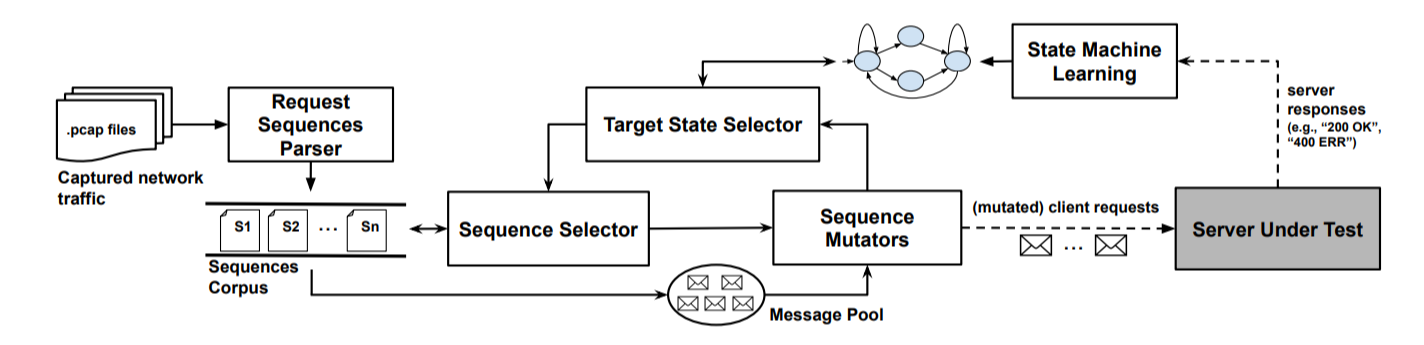
\includegraphics[width=15cm]{images/aflnet.png}
    \label{fig:1}
    \captionsetup{justification=centering,margin=1cm}
    \captionof{figure}{AFLNet Architecture}
\end{center}
\vspace{0.3cm}

\section{Proof of Concept}

For testing the applicability of fuzzing in the network protocols security testing, two approaches were adopted. Firstly, we tested a \textbf{custom C application} that implements a custom protocol with a blackbox, smart fuzzer, namely \textbf{boofuzz}. Secondly, an \textbf{open source project} was tested with a greybox, dumb fuzzer, namely \textbf{AFLNet}. Both approaches shown that the vulnerability, that we deliberately introduced in the SUTs, were discovered by the two fuzzers.

\subsection{boofuzz}

For this example, we have implemented a custom TCP protocol that can write/retrieve data to/from a file.

The protocol structure is the following. The client must first send a packet containing the username. The second packet that the user has to send after contains his choice whether to write to a file or to read from it, after specifying an option the client can then provide an arbitrary filename. If the read method is selected, the server will return the specified file contents. If the write method is used, the server will wait for a third packet in which the client can send the desired data to be written. 

All operations are marked as complete by the server with an \mintinline{text}{END} message that is sent to the client. We have used this mechanism of marking as complete an operation as a method to detect if errors occurred in the server.

For this proof of concept, we have used boofuzz as its code is available on GitHub \cite{boofuzz_repo}. Inside the Python 3 script, we create a \mintinline{text}{Session} object as this is responsible for tracking the requests, callbacks and server state. The next step is defining the protocol as two primitives (\mintinline{text}{Blocks} method inside boofuzz, one for each scenario), setting fuzzable fields and static ones (such like the newline after each packet from the client). Then we define a custom callback function that receives data from the server and checks for the special message to mark an operation as complete, if a certain amount of time has elapsed or the special message is not present, then we consider marking the case as a favorable one with the help of the logging mechanism provided by the fuzzer. No process monitor was used for this proof of concept, instead a Bash script that reopens the server process was used.

\subsection{AFLNet}

The repository of the AFLNet contains a \mintinline{text}{Dockerfile} used for fuzzing an FTP server, LightFTP\footnote{\href{https://github.com/aflnet/aflnet/blob/master/tutorials/lightftp/Dockerfile}{https://github.com/aflnet/aflnet/blob/master/tutorials/lightftp/Dockerfile}}. It was downloaded and used as a base for the fuzzing process that will be described above. In addition, the operating system was updated (with another one supported by AFLNet), some dependencies were added (including LLVM 6.0) and the section targeting LightFTP was removed. The image was then built, and a \textbf{test container} created.

We choose an open source project to fuzz, namely \textbf{CivetWeb}, which is a C embeddable web server. Its GitHub repository was cloned, and the binaries were compiled with AFL instrumentation and installed in the host operating system. After this, the logging was enabled (to be able to trace the fuzzer actions) and a script created to ensure the server restart after a crash. The latter is due to the fact that if a request produces a crash, it will propagate to the whole process.

We recorded in binary format multiple valid requests with \textbf{Wireshark}. A filter was configured for HTTP and for the destination IP address, which is the container's one. In addition, the \textbf{dictionaries} made available in the sources of CivetWeb \footnote{\href{https://github.com/civetweb/civetweb/blob/master/fuzztest/http1.dict}{https://github.com/civetweb/civetweb/blob/master/fuzztest/http1.dict}} were passed to the fuzzer such that the latter could benefit for having a structure. As these were the last requirements that needs to be fulfilled, AFLNet was then started and the application fuzzed for several minutes.

The mutation that the fuzzer does can be seen in the \textbf{log file}, as in the examples made available in the GitHub repository \cite{project_repo}. We observed such mutations on the path that the request targets and on the user agent.

As no vulnerability was discovered in the given amount of time, we wanted to prove that our method was correct. A \textbf{new vulnerable function} was introduced in the source code of CivetWeb, which transforms to lowercase all the letters of the user agent found in requests using a buffer with a fixed size. If the user agent exceeds it, a heap buffer overflow is triggered. In this case, AFLNet was able to crash the SUT in several seconds, validating the initial fuzzing session.

\section{Detection. Countermeasures}

The fuzzing approach for finding vulnerabilities could be used not only by the software developers and the
product security teams, but by the attackers too. By sending numerous requests to a local or remote server, a threat actor could detect security bugs, which could bring him powerful capabilities: reading and altering user data, executing code or disrupting the functionality of production servers.

\textbf{This risk needs to be mitigated} by the software development teams by binding out methods for protecting their software. In this chapter, there will be presented some anti-fuzzing techniques and, in general, ones for defending software that relies on networking for their functioning.

\subsection{Anti-Fuzzing Techniques}

In 2019, at USENIX Security Symposium, the paper "\textit{ANTIFUZZ: Impeding Fuzzing Audits of Binary Executables}" \cite{antifuzz} was presented. Multiple fuzzers were analyzed and some fundamental assumptions (such as the fact that the crashes can be detected and that many executions can be performed per second) were identified, without which the fuzzing process is impossible or, minimally, slowed down.

In the context of network fuzzing, some techniques can be applied. An example is an \textbf{artificially-induced delay for malformed requests}, that are created automatically by a fuzzer. If the server detects that a request does not respect the standard format (for example, an unknown protocol type in a TCP packet), it will respond only after a delay, which will reflect into the speed of the fuzzing process too.

\subsection{Rate Limiting}

Rate limiting is another strategy for decreasing the performance of automated tools. It relies on \textbf{setting a limit of requests} to the server, for a given client. The latter is identified by a unique number in the protocol format. These can appear at different layers in the ISO/OSI model and can vary from IP addresses (transport layer) to cookies in HTTP (application layer).

These techniques manage to mitigate attacks such as fuzzing, brute force attacks, (distributed) denial of service and scraping, in which the result of the attack is directly proportional with the number of received responses.

\subsection{Crash Reporting}

The last technique that needs to be mentioned is crash reporting. Additional code needs to be inserted in the program (in this case, the SUT) or in the host operating system. If the application crashes, it will record information about the state of the process and send it to a central server, where these \textbf{crash dumps are collected and analyzed} by the specialized personnel of the software provider.

For network protocols, all the data that is received by the server needs to be recorded via the techniques mentioned above or via a \textbf{full-packet capture} on the network (or on SUT). This scenario can impose additional difficulties due to the process of correlating the network packets with the exact data that triggered the crash.

\section{Related Work}

As described in the introductory chapter, the network protocol are, in fact, only sequences of bytes used by programs running on different computers (or on the same computer, speaking in terms of inter-process communication via sockets). So a vulnerability in a network protocol is, at its root, a vulnerability in the mentioned program.

In this chapter, it will be described \textbf{alternative techniques}, \textbf{researched intensively in the academia} and \textbf{applied with success in industry}, that can be used to target the same goal.

\subsection{Code Review}

When the source code is accessible, a task that could be accomplished by a software provider or an attacker is reviewing it. This implies a code traverse, line by line, and finding the ones which present a security risk. The advantage of this method is that all the operations are static, not involving a run of the SUT.

The process could be either manual, as practiced on the bug bounty community or by attackers, when targeting open source projects, or automated. For examples, Snyk\footnote{\href{https://snyk.io}{https://snyk.io}} could be used as a platform for finding vulnerabilities in software products. It offers both free and paid services, depending on the scope of the product and the size of the development team. On the other hand, there is also GitHub Dependabot which scans the open source repositories for dependencies and send weekly emails to the owners, recalling that updates are needed\footnote{\href{https://github.com/dependabot/dependabot-core}{https://github.com/dependabot/dependabot-core}}.

In the protocols' security scenario, the reviewer (human or automated scanner) needs to pay \textbf{attention to all the networking operations}, from the aspects regarding the encryption and authentication of the parties communicating to the processing of the received data, namely checking the validation strategy.

\subsection{Taint Analysis}

Taint analysis refers to defining an untrusted source of data (in the networking scope, the requests' data processed by SUT), marking the data propagated from that source as tainted and detecting whether it is further used in dangerous ways. For instance, is the SUT has a stack buffer that could be overwritten by data received from a socket, a taint analysis tool can \textbf{detect} if relevant stack data (saved base pointer, return address) are altered and trigger an alert that could be then patched by the developers.

Besides the above-presented scenario, in which the analysis of the tainted data could indicate what part of the packet triggered the vulnerability, there is another significant usage: \textbf{extraction of message format from protocol implementation}. So a blackbox fuzzer, which does not have access to many details of the testing scenario, could gradually build the grammar used in packets generation, despite the fact this was not explicitly mentioned \cite{polyglot}.

\subsection{Symbolic Execution}

Symbolic execution helps on finding the edge cases in which a program could behave incorrectly. It uses a \textbf{representation of the program inputs} (arguments, \mintinline{text}{stdin}, network data) \textbf{as symbolic} and a propagation of these into other variables. In contract to dynamic taint analysis, which only states that a vulnerability was triggered, symbolic execution can find them proactively.

As an example, there were proposed novel approaches that leverages the symbolic execution to test binaries implementing network protocols \cite{symex_protocols}. In the cited paper, the provided method was able to detect known vulnerabilities in two targets implementing HTTP and FTP.

\subsection{Formal Validation}

The last method for finding vulnerabilities in the network context is by formal validation. This method relies on mathematical models to verify its \textbf{absolute logical correctness}. In academia, some papers verifies well-known forwarding \cite{formal_verification_bgp}, such as BGP, and IoT protocols \cite{formal_verification_iot}.

\section{Conclusions}

This paper demonstrates that the fuzzing, a technique used mainly for finding vulnerabilities in binaries, can be used with success for finding vulnerabilities in network protocols. This is possible because the network protocols are, at their root, only a mean by which processes (from the same host, via internal sockets, or externally, in a LAN) communicates in a structured way.

We offered two proof of concepts: one targeting a custom protocol (replaying on TCP) from a custom application with a blackbox smart fuzzer, boofuz, and another targeting an open source embeddable web server with a graybox dumb fuzzer, AFLNet. In the latter case, as no vulnerability was discovered, we manually introduced a heap buffer overflow in the processing of the user agent. In both scenarios, the fuzzers were able to detect the deliberately-introduced vulnerabilities from SUTs.

Lastly, fuzzing is an effective  way to detect vulnerabilities in network protocols. Despite the fact that the SUTs response speed can be limited by the binary instrumentation, the ongoing research can adjust this. In any case, this integration is quite pragmatic, but will never outpace a formal validation, in which the logic and the implementation of a protocol can be proven theoretically.

% Bibliography
\section{Bibliography}
\nocite{*}
\printbibliography[heading=none]

\end{document}